
\section{Overview}

The Global Arrays toolkit has recently been extended to support global
arrays defined on processor groups. The processor groups in GA programs
follow the MPI approach. The MPI processor groups can be used in GA
programs. However, since the MPI standard does not support fault tolerance,
GA provides a set of APIs for process group managment which offers
some opportunities for supporting environments with hardware faults.

In general, processor groups allow the programmer to subdivide the
domain containing the complete set of processors (\textquotedblleft{}the
world group\textquotedblright{}) into subsets of processors that can
act more or less independently of one another. Global arrays that
are created on processor groups are only distributed amongst the processors
in the group and not on all processors in the system. Collective operations
executed on specific groups are also restricted to processors in the
group and do not require any action from processors outside the group.
A simple example is a synchronization operation. If the synchronization
operation is executed on a group that is a subgroup of the world group,
then only those processors in the subgroup are blocked until completion
of the synchronization operation. Processors outside the subgroup
can continue their operations without interruption.

The Global Arrays toolkit contains a collection of library calls that
can be used to explicitly create groups, assign specific groups to
global arrays, and execute global operations on groups. There is also
a mechanism for setting the \textquotedblleft{}default\textquotedblright{}
group for the calculation. This is a powerful way of converting large
amounts of parallel code that has already been written using the Global
Arrays library to run as a subroutine on a processor group. Normally,
the default group for a parallel calculation is the world group, but
a call is available that can be used to change the default group to
something else. This call must be executed by all processors in the
subgroup. Furthermore, although it is not required, it is probably
a very good idea to make sure that the default groups for all processors
in the system (i.e., all processors contained in the original world
group) represent a complete non-overlapping covering of the original
world group (see figure). Once the default group has been set, all
operations are implicitly assumed to occur on the default processor
group unless explicitly stated otherwise. Global Arrays are only created
on the default processor group and global operations, such as synchronizations,
broadcasts, and other operations, are restricted to the default group.
Inquiry functions, such as the number of nodes and the node ID, return
values relative to the default processor group. Thus, a call to the
ga\_nodeid function will return a value of 0 for each processor designated
as the zero processor within each default group. The number of processors
returning 0 will be equal to the number of default groups (assuming
the complete non-overlapping coverage suggested above is implemented).

\begin{tabular}{|>{\centering}p{10cm}|}
\hline 
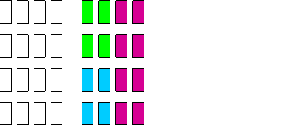
\includegraphics{groups}\tabularnewline
\hline
\hline 
Original set of 16 processors decomposed into 3 non-overlapping groups.\tabularnewline
\hline
\end{tabular}

At present there are not many function calls that support operations
between groups. The only calls that can be used to copy data from
one group to another are the \texttt{nga\_copy} and \texttt{nga\_copy\_patc}h
calls. These can be used to copy global arrays between two groups,
provided that one group is completely contained in the other (this
will always be the case if one of the groups is the world group).
These commands will work correctly as long as they are executed only
by processors contained in the smaller group. The \texttt{nga\_put}
and \texttt{nga\_get} commands can also be used to communicate between
Global Arrays on different groups (using an intermediate buffer),
provided that the two groups share at least one processor (again,
this will always be the case if one group is the world group).

The new functions included in the Global Arrays library are described
below. 


\section{Creating New Groups}
\begin{lyxcode}
\textcolor{blue}{Fortran}~integer~function~\href{http://www.emsl.pnl.gov/docs/global/ga_ops.html\#GA_PGROUP_CREATE}{ga\_{}pgroup\_{}create}(list,~size)

\textcolor{blue}{C}~~~~~~~int~\href{http://www.emsl.pnl.gov/docs/global/c_nga_ops.html\#GA_PGROUP_CREATE}{GA\_{}Pgroup\_{}create}(int~{*}list,~int~size)
\end{lyxcode}
This call can be used to create a processor group of size \texttt{size}
containing the processors in the array \texttt{list}. This call must
be executed on all processors in the group. It returns an integer
handle (for the processors group) that can be used to reference the
processor group in other library calls.

Assigning groups:
\begin{lyxcode}
\textcolor{blue}{Fortran}~subroutine~\href{http://www.emsl.pnl.gov/docs/global/ga_ops.html\#GA_SET_PGROUP}{ga\_{}set\_{}pgroup}(g\_a,~p\_handle)

\textcolor{blue}{C}~~~~~~~void~\href{http://www.emsl.pnl.gov/docs/global/c_nga_ops.html\#GA_SET_PGROUP}{GA\_{}Set\_{}pgroup}(int~g\_a,~int~p\_handle)
\end{lyxcode}
This call can be used to assign the processor group \texttt{p\_handle}
to a global array handle \texttt{g\_a} that has been previously created
using the \texttt{ga\_create\_handle} call. The processor group associated
with a global array can also be set by creating the global array with
one of the \texttt{nga\_create\_XXX\_config} calls. 


\section{Setting the Default Group}
\begin{lyxcode}
\textcolor{blue}{Fortran}~subroutine~\href{http://www.emsl.pnl.gov/docs/global/ga_ops.html\#GA_PGROUP_SET_DEFAULT}{ga\_{}pgroup\_{}set\_{}default}(p\_handle)

\textcolor{blue}{C}~~~~~~~void~\href{http://www.emsl.pnl.gov/docs/global/c_nga_ops.html\#GA_PGROUP_SET_DEFAULT}{GA\_{}Pgroup\_{}set\_{}default}(int~p\_handle)
\end{lyxcode}
This call can be used to set the default group to something besides
the world group. This call must be made on all processors contained
in the group represented by \texttt{p\_handle}. Once the default group
has been set, all operations are restricted to the default group unless
explicitly stated otherwise. 


\section{Inquiry functions}
\begin{lyxcode}
\textcolor{blue}{Fortran}~integer~function~\href{http://www.emsl.pnl.gov/docs/global/ga_ops.html\#GA_PGROUP_NNODES}{ga\_{}pgroup\_{}nnodes}(p\_handle)

\textcolor{blue}{C}~~~~~~~int~\href{http://www.emsl.pnl.gov/docs/global/c_nga_ops.html\#GA_PGROUP_NNODES}{GA\_{}Pgroup\_{}nnodes}(int~p\_handle)

\textcolor{blue}{Fortran}~integer~function~\href{http://www.emsl.pnl.gov/docs/global/ga_ops.html\#GA_PGROUP_NODEID}{ga\_{}pgroup\_{}nodeid}(p\_handle)

\textcolor{blue}{C}~~~~~~~int~\href{http://www.emsl.pnl.gov/docs/global/c_nga_ops.html\#GA_PGROUP_NODEID}{GA\_{}Pgroup\_{}nodeid}(int~p\_handle)
\end{lyxcode}
These functions can be used to access information about the group.
The \texttt{ga\_pgroup\_nnodes} function returns the number of processors
in the group specified by the handle \texttt{p\_handle}, \texttt{ga\_pgroup\_nodeid}
returns the local node ID of the processor within the group.
\begin{lyxcode}
\textcolor{blue}{Fortran}~integer~function~\href{http://www.emsl.pnl.gov/docs/global/ga_ops.html\#GA_PGROUP_GET_DEFAULT}{ga\_{}pgroup\_{}get\_{}default}()

\textcolor{blue}{C}~~~~~~~int~\href{http://www.emsl.pnl.gov/docs/global/c_nga_ops.html\#GA_PGROUP_GET_DEFAULT}{GA\_{}Pgroup\_{}get\_{}default}()

\textcolor{blue}{Fortran}~integer~function~\href{http://www.emsl.pnl.gov/docs/global/ga_ops.html\#GA_PGROUP_GET_MIRROR}{ga\_{}pgroup\_{}get\_{}mirror}()

\textcolor{blue}{C}~~~~~~~int~\href{http://www.emsl.pnl.gov/docs/global/c_nga_ops.html\#GA_PGROUP_GET_MIRROR}{GA\_{}Pgroup\_{}get\_{}mirror}()

\textcolor{blue}{Fortran}~integer~function~\href{http://www.emsl.pnl.gov/docs/global/ga_ops.html\#GA_PGROUP_GET_WORLD}{ga\_{}pgroup\_{}get\_{}world}()

\textcolor{blue}{C}~~~~~~~int~\href{http://www.emsl.pnl.gov/docs/global/c_nga_ops.html\#GA_PGROUP_GET_WORLD}{GA\_{}Pgroup\_{}get\_{}world}()
\end{lyxcode}
These functions can be used to get the handles for some standard groups
at any point in the program. This is particularly useful for gaining
access to the world group if the default group has been reset to a
subgroup and also for gaining access to the handle for the mirror
group (see section on mirrored arrays). Note that the mirror group
is actually a group defined on the complete set of processors. 


\section{Collective operations on groups}
\begin{lyxcode}
\textcolor{blue}{Fortran}~subroutine~\href{http://www.emsl.pnl.gov/docs/global/ga_ops.html\#GA_PGROUP_SYNC}{ga\_{}pgroup\_{}sync}(p\_handle)

\textcolor{blue}{C}~~~~~~~void~\href{http://www.emsl.pnl.gov/docs/global/ga_ops.html\#GA_PGROUP_SYNC}{ga\_{}pgroup\_{}sync}(p\_handle)

\textcolor{blue}{Fortran}~subroutine~\href{http://www.emsl.pnl.gov/docs/global/ga_ops.html\#GA_PGROUP_BRDCST}{ga\_{}pgroup\_{}brdcst}(p\_handle,type,

~~~~~~~~~~~~~~~~~~~buf,lenbuf,root)

\textcolor{blue}{C}~~~~~~~void~\href{http://www.emsl.pnl.gov/docs/global/ga_ops.html\#GA_PGROUP_BRDCST}{GA\_{}Pgroup\_{}brdcst}(int~p\_handle,~void~

~~~~~~~~~~~~~~~~~~~{*}buf,~root)

\textcolor{blue}{Fortran}~subroutine~\href{http://www.emsl.pnl.gov/docs/global/ga_ops.html\#GA_PGROUP_DGOP}{ga\_{}pgroup\_{}dgop}(p\_handle,~type,~

~~~~~~~~~~~~~~~~~~~buf,~lenbuf,~op)

\textcolor{blue}{Fortran}~subroutine~\href{http://www.emsl.pnl.gov/docs/global/ga_ops.html\#GA_PGROUP_SGOP}{ga\_{}pgroup\_{}sgop}(p\_handle,~type,~

~~~~~~~~~~~~~~~~~~~buf,~lenbuf,~op)

\textcolor{blue}{Fortran}~subroutine~\href{http://www.emsl.pnl.gov/docs/global/ga_ops.html\#GA_PGROUP_IGOP}{ga\_{}pgroup\_{}igop}(p\_handle,~type,~

~~~~~~~~~~~~~~~~~~~buf,~lenbuf,~op)

\textcolor{blue}{C}~~~~~~~void~\href{http://www.emsl.pnl.gov/docs/global/c_nga_ops.html\#GA_PGROUP_DGOP}{GA\_{}Pgroup\_{}dgop}(int~p\_handle,~double~

~~~~~~~~~~~~~~~~~~~{*}buf,~int~lenbuf,~char~{*}op)

\textcolor{blue}{C}~~~~~~~void~\href{http://www.emsl.pnl.gov/docs/global/c_nga_ops.html\#GA_PGROUP_FGOP}{GA\_{}Pgroup\_{}fgop}(int~p\_handle,~float~

~~~~~~~~~~~~~~~~~~~{*}buf,~int~lenbuf,~char~{*}op)

\textcolor{blue}{C}~~~~~~~void~\href{http://www.emsl.pnl.gov/docs/global/c_nga_ops.html\#GA_PGROUP_IGOP}{GA\_{}Pgroup\_{}igop}(int~p\_handle,~int~

~~~~~~~~~~~~~~~~~~~{*}buf,~int~lenbuf,~char~{*}op)

\textcolor{blue}{C}~~~~~~~void~\href{http://www.emsl.pnl.gov/docs/global/c_nga_ops.html\#GA_PGROUP_LGOP}{GA\_{}Pgroup\_{}lgop}(int~p\_handle,~long~

~~~~~~~~~~~~~~~~~~~{*}buf,~int~lenbuf,~char~{*}op)
\end{lyxcode}
These operations are all identical to the standard global operations,
the only difference is that they have an extra argument that takes
a group handle. The action of these calls is restricted to the set
of processors contained in the group represented by \texttt{p\_handle}.
All processors in the group must call these subroutines.
